\chapter{editor\_learnerの概要}

    \section{Installation}\label{installation}

\subsection{githubによるinstall}\label{githubux306bux3088ux308binstall}

githubによるインストール方法は以下の通りである.

\begin{enumerate}
\def\labelenumi{\arabic{enumi}.}
\tightlist
\item
  "https://github.com/souki1103/editor\_learner" へアクセス
\item
  Clone or downloadを押下,SSHのURLをコピー
\item
  コマンドラインにてgit clone(コピーしたURL)を行う
\end{enumerate}

上記の手順で開発したファイルがそのまま自分のディレクトリにインストールされる.

\subsection{gemによるinstall}\label{gemux306bux3088ux308binstall}

gemによるインストール方法は以下の通りである.

\begin{enumerate}
\def\labelenumi{\arabic{enumi}.}
\tightlist
\item
  コマンドラインにてgem install editor\_learnerと入力,実行
\item
  ファイルがホームディレクトの.rbenv/versions/2.4.0/lib/ruby/gems/2.4.0/gemsにeditor\_learnerが収納される
\end{enumerate}

これでeditor\_learnerとコマンドラインで入力することで実行可能となる.

    \section{uninstall}\label{uninstall}

\subsection{githubからinstallした場合のuninstall方法}\label{githubux304bux3089installux3057ux305fux5834ux5408ux306euninstallux65b9ux6cd5}

gituhubからinstallした場合のuninstall方法は以下の通りである.

\begin{enumerate}
\def\labelenumi{\arabic{enumi}.}
\tightlist
\item
  ホームディレクトで

  \begin{enumerate}
  \def\labelenumii{\arabic{enumii}.}
  \tightlist
  \item
    rm -rf editor\_learnerを入力
  \end{enumerate}
\item
  ホームディレクトリからeditor\_learnerが削除されていることを確認する.
\end{enumerate}

以上がuninstall方法である.

\subsection{gemからinstallした場合のuninstall方法}\label{gemux304bux3089installux3057ux305fux5834ux5408ux306euninstallux65b9ux6cd5}

gemからinstallした場合のuninstall方法は以下の通りである.

\begin{enumerate}
\def\labelenumi{\arabic{enumi}.}
\tightlist
\item
  ターミナル上のコマンドラインで

  \begin{enumerate}
  \def\labelenumii{\arabic{enumii}.}
  \tightlist
  \item
    gem uninstall editor\_learnerを入力
  \end{enumerate}
\item
  ホームディレクトの.rbenv/versions/2.4.0/lib/ruby/gems/2.4.0/gemsにeditor\_learnerが削除されていることを確認する.
\end{enumerate}

以上がuninstall方法である.

    \section{動作環境}\label{ux52d5ux4f5cux74b0ux5883}

    Rubyのversionが2.4.0以上でなければ動かない.理由としては,gemに格納されているパスを正しいく受け渡しできないからである.2.4.0以下で動作させるためにはeditor\_learnerの最新versionのみを入れることによって動作することが確認できている.

\subsection{error時の対処法}\label{errorux6642ux306eux5bfeux51e6ux6cd5}

errorが出た場合は以下の方法を試してください

\begin{enumerate}
\def\labelenumi{\arabic{enumi}.}
\tightlist
\item
  rm -rf editor\_learnerをコマンドラインで入力
\end{enumerate}

これによりファイル生成によるバグを解消できる.もう一つの方法は

\begin{enumerate}
\def\labelenumi{\arabic{enumi}.}
\tightlist
\item
  gem uninstall editor\_learnerをコマンドラインで入力
\item
  全てのversionをuninstallする.
\item
  再度gem install editor\_learnerで最新versionのみをinstallする.
\end{enumerate}

上記の手順によりRubyのversionによるバグが解消されることが確認できている.現在起こるであろうと予想されるバグの解消法は上記の2つである.Rubyのversionが2.4.0以上であればなんの不具合もなく動作することが確認できている.

    \section{初期設定}\label{ux521dux671fux8a2dux5b9a}

    特別な初期設定はほとんどないが起動方法は以下の通りである,

\begin{enumerate}
\def\labelenumi{\arabic{enumi}.}
\tightlist
\item
  コマンドライン上にてeditor\_learnerを入力する.

  \begin{enumerate}
  \def\labelenumii{\arabic{enumii}.}
  \setcounter{enumii}{1}
  \tightlist
  \item
    editor\_learnerを起動することでホームディレクトリにeditor\_learner/workshopと呼ばれるファイルが作成される.workshopは作業場という意味である.
  \item
    workshopの中にquestion.rbとanswer.rb,random\_h.rbとruby\_1~ruby\_6が作成され,ruby\_1ruby\_6の中に1.rb~3.rbが作成されていることを確認する.
  \end{enumerate}
\end{enumerate}

\begin{figure}[H]
\centering
\begin{center}
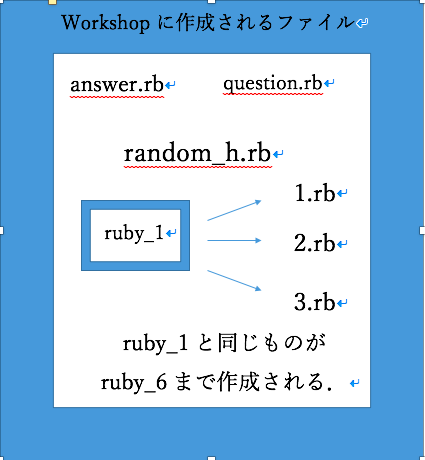
\includegraphics[width=150mm]{../../picture/mkdir.png}
\end{center}
\caption{作られるファイルの説明.\label{sample}}

\label{fig:This}
\end{figure}

\begin{enumerate}
\def\labelenumi{\arabic{enumi}.}
\item
  起動すると以下のようなサブコマンドの書かれた画面が表示されることを確認する.

\begin{verbatim}
Commands:
editor_lerner delete [number~number]
editor_learner help [COMMAND]
editor_learner random_check
editor_leraner sequential_check [lesson_number] [1~3numbers]
\end{verbatim}
\item
  editor\_learnerの後にサブコマンドと必要に応じた引数を入力すると動作する.それぞれのサブコマンドの更に詳しい説明は以下の通りである.
\end{enumerate}

    \section{delete}\label{delete}

    editor\_learnerを起動することで初期設定で述べたようにホームディレクトリにeditor\_learner/workshopが作成される.deleteはworkshopに作成されたruby\_1\textasciitilde{}ruby\_6を削除するために作成されたものである.sequential\_checkで1度プログラムを作成してしまうと再度実行するとIt
have been
finished!と表示されてしまうので,削除するコマンドを作成しました.コマンド例は以下の通りである.

コマンド例

\begin{enumerate}
\def\labelenumi{\arabic{enumi}.}
\tightlist
\item
  editor\_learner delete 1 3
\end{enumerate}

上記のように入力することで1〜3までのファイルが削除される.サブコマンドの後の引数は2つの数字(char型)であり,削除するファイルの範囲を入力する.

    \section{random\_h.rbとsequential\_h.rb}\label{random_h.rbux3068sequential_h.rb}

random\_h.rbとsequential\_h.rbが初期設定で作成され,editor\_learnerを起動することで自動的に作成され,random\_checkとsequential\_checkを行う際に最初に開くファイルとなる.random\_check用とsequential\_check用に二つのファイルがある.random\_check用のファイルは以下の通りである.

random\_h.rb

\begin{figure}[H]
\centering
\begin{center}
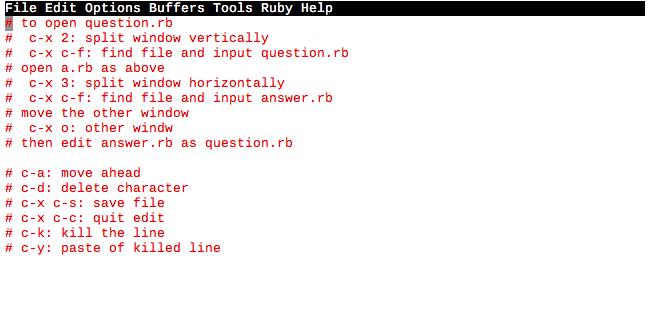
\includegraphics[width=150mm]{../../picture/random_h.png}
\end{center}
\caption{random\_h.rb.\label{random_h}}

\label{fig:}
\end{figure}

上から順に説明すると,
\begin{enumerate}
\def\labelenumi{\arabic{enumi}.}
\tightlist
\item
question.rbを開くためにc-x2で画面を2分割にする.
\item
c-x c-fでquestion.rbのパスを入力して開く. 
\item
次にanswer.rbを開くために画面を3分割する 
\item
同様にc-x c-fでanswer.rbのパスを入力して開く. 
\item
c-x oでanswer.rbを編集するためにポインタを移動させる. 
\item
question.rbに書かれているコードをanswer.rbに写す.
\end{enumerate}
これらの手順がrandom\_h.rbに記述されている.全ての手順を終えたターミナルの状態は以下の通り,

\begin{figure}[H]
\centering
\begin{center}
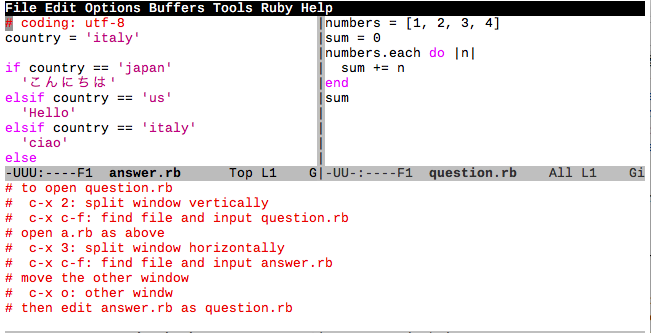
\includegraphics[width=150mm]{../../picture/split.png}
\end{center}
\caption{全ての操作を終えたターミナル画面.\label{split}}

\label{fig:}
\end{figure}

上記の画像では,右上に問題であるquestion.rbが表示され,それを左上にあるanswer.rbに写す形となる.

次にsequential\_h.rb

\begin{figure}[H]
\centering
\begin{center}
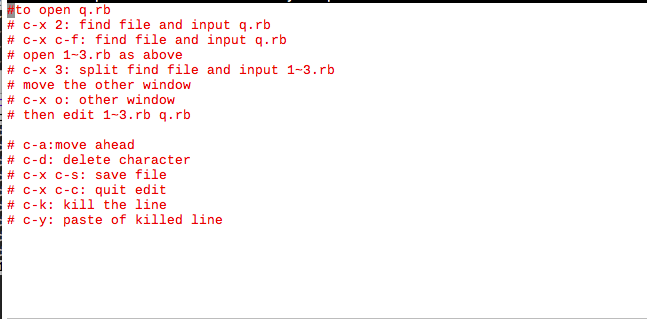
\includegraphics[width=150mm]{../../picture/sequential_h.png}
\end{center}
\caption{sequential\_h.rb.\label{sqquential}}

\label{fig:}
\end{figure}

書かれている内容自体はrandom\_h.rbとほとんど差異がないが,開くファイルの名前が違うため別のファイルとして作成された.この手順に沿って作業することになる.下に書かれているのは主要キーバインドであり,必要に応じて見て,使用する形となっている.上記の手順を行なったターミナル画面の状態はrandom\_h.rbの最終形態を同じである.

    \section{random\_checkの動作}\label{random_checkux306eux52d5ux4f5c}

random\_checkの動作開始から終了は以下の通りである.

\begin{enumerate}
\def\labelenumi{\arabic{enumi}.}
\tightlist
\item
  コマンドライン上にてeditor\_learne random\_checkを入力
\item
  新しいターミナル(ホームディレクトリ/editor\_learner/workshopから始まる)が開かれる.
\item
  random\_h.rbを開いてrandom\_h.rbに沿ってquestion.rbに書かれているコードをanswer.rbに写す.
\item
  前のターミナルに戻り,コマンドラインに"check"と入力することで正誤判定を行ってくれる.
\item
  間違っていればdiff-lcsにより間違った箇所が表示される.
\item
  正しければ新しいターミナルが開かれてから終了までの時間とIt have been
  finished!が表示され終了となる.
\end{enumerate}

更に次回random\_check起動時には前に書いたコードがanswer.rbに格納されたままなので全て削除するのではなく,前のコードの必要な部分は残すことができる.

random\_checkの大きな目的はtyping速度,正確性の向上,editor操作やRuby言語の習熟に重点を置いている.いかに早く終わらせるかのポイントがtyping速度,正確性とeditor操作である.

    \section{sequential\_checkの動作}\label{sequential_checkux306eux52d5ux4f5c}

    sequential\_checkの動作開始から終了は以下の通りである.

\begin{enumerate}
\def\labelenumi{\arabic{enumi}.}
\tightlist
\item
  コマンドライン上でeditor\_learner
  sequential\_check(1\textasciitilde{}6の数字)
  (1\textasciitilde{}3の数字)を入力
\item
  新しいターミナル(ホームディレクトリ/editor\_learner/workshop/ruby\_(1\textasciitilde{}6の数字))が開かれる.
\item
  sequential\_h.rbを開いてsequential\_h.rbに沿ってq.rbに書かれている内容を第2引数の数字.rbに写す.
\item
  前のターミナルに戻り,コマンドラインに"check"と入力することで正誤判定を行う.
\item
  間違っていれば間違った箇所が表示される.再度q.rbと第2引数の数字.rbを開いて間違った箇所を修正する.
\item
  正しければruby\_1/1.rb is done!のように表示される.
\end{enumerate}

sequential\_checkは1\textasciitilde{}3の順に1.rbがリファクタリングや追加され2.rbになり,完成形が3.rbになるといった形式である.連続的なプログラムの完成までを写経するのでsequential\_checkと名付けられた.

sequential\_checkの大きな目的はリファクタリングによるRuby言語の学習とCUI操作によるキーバインドの習熟,タイピング速度,正確性の向上に重点を置いている.コードがリファクタリングされる様を写経することで自分自身でRubyのコードを書くときに他の人が見やすくなるようなコードが書けるようになる.